\documentclass[../../thesis.tex]{subfiles}


\begin{document}
    \begin{figure}[H]
        \centering
        \subfloat[]{
        \tikzsetnextfilename{production_stage_1}
            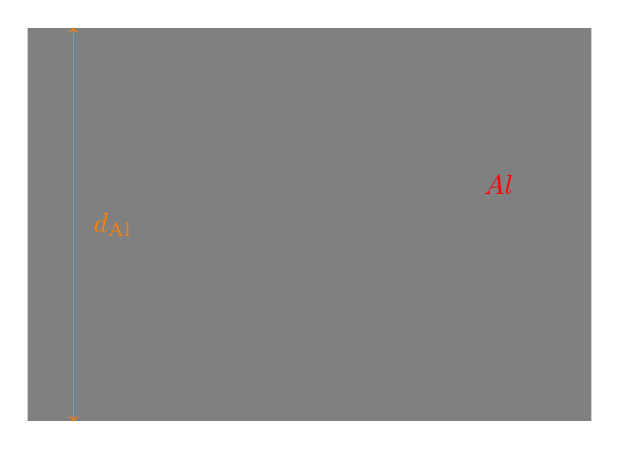
\begin{tikzpicture}
                \def\l{7.2};
                \def\h{5};
                \def\d{0.8};
                \begin{scope}
                    \clip (0.02,0) rectangle (\l - 0.02,\h);
                    \fill[gray] (0,0) rectangle (\l,\h);
                    \draw[color=orange,<->] (0.6,0) -- (0.6,\h);
                    \node[color=orange] at (1.1,\h/2) {$d_\mathrm{Al}$};
                    \node[color=red] at (6,3) {$\ce{Al}$};
                \end{scope}
            \end{tikzpicture}
            \label{fig:bulk-al}}
        \hfill
        \subfloat[]{
        \tikzsetnextfilename{production_stage_2}
            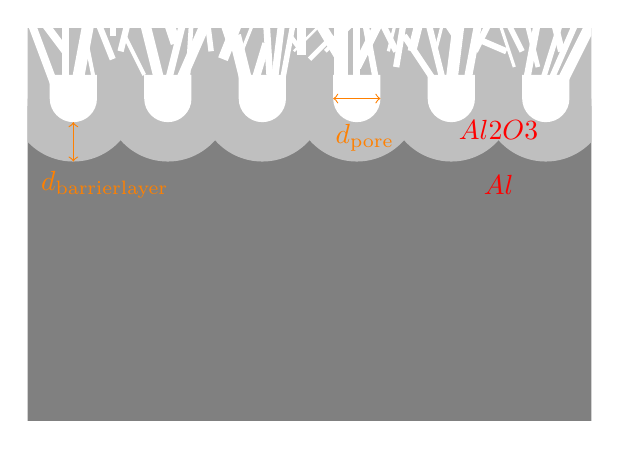
\begin{tikzpicture}
                \def\l{7.2};
                \def\h{5};
                \def\d{0.6};
                \begin{scope}
                    \clip (0.02,0) rectangle (\l - 0.02,\h);
                    \fill[gray] (0,0) rectangle (\l,\h-1);
                    \fill[lightgray] (0,\h-1) rectangle (\l,\h);
                    \foreach \i in {1,3,...,11}{
                        \fill[lightgray] (- 4 / 3 * \d + \i * \d, \h - 1 + 0.1) arc (180:360:\d / 3 * 4);
                        \fill[white] (-0.5 * \d + \i * \d, \h - 1 + 0.1) arc (180:360:\d / 2) -- (-0.5 * \d + \i * \d + \d, \h - 0.7 + 0.1) -- (-0.5 * \d + \i * \d, \h - 0.7 + 0.1) -- cycle;}
                        \begin{scope}[yshift = 2cm]
                            \draw[color=white, line width=1mm] (0.2,3.1) -- (0.5,2.7);
                            \draw[color=white, line width=1mm] (0.5,3.1) -- (0.5,2.3);
                            \draw[color=white, line width=1mm] (0.05,3.1) -- (0.35,2.3);
                            \draw[color=white, line width=1.5mm] (0.8,3.1) -- (0.65,2.3);
                            \draw[color=white, line width=0.5mm] (0.75,2.9) -- (0.87,2.3);
                            \draw[color=white, line width=0.8mm] (0.9,3.1) -- (1.1,2.6);
                            \draw[color=white, line width=0.8mm] (1.1,3.1) -- (1.1,2.9);
                            \draw[color=white, line width=0.8mm] (1.3,3.1) -- (1.2,2.7);
                            \draw[color=white, line width=0.5mm] (1.25,2.9) -- (1.5,2.4);
                            \draw[color=white, line width=1.3mm] (1.5,3.1) -- (1.7,2.3);
                            \draw[color=white, line width=1.3mm] (1.8,3.1) -- (1.9,2.8);
                            \draw[color=white, line width=0.6mm] (2.1,3.1) -- (2.05,2.3);
                            \draw[color=white, line width=0.9mm] (2,3.1) -- (1.8,2.3);
                            \draw[color=white, line width=1.3mm] (2.3,3.1) -- (1.95,2.3);
                            \draw[color=white, line width=0.7mm] (2.3,3.1) -- (2.35,2.7);
                            \draw[color=white, line width=1mm] (2.5,3.1) -- (2.6,2.8);
                            \draw[color=white, line width=1.3mm] (2.7,3.1) -- (2.5,2.6);
                            \draw[color=white, line width=1.6mm] (2.65,2.9) -- (2.8,2.3);
                            \draw[color=white, line width=0.4mm] (2.9,3.1) -- (2.7,2.6);
                            \draw[color=white, line width=0.86mm] (3.05,3.1) -- (3.1,2.3);
                            \draw[color=white, line width=1mm] (3.05,2.8) -- (2.9,2.3);
                            \draw[color=white, line width=0.9mm] (3.25,3.1) -- (3.15,2.3);
                            \draw[color=white, line width=0.7mm] (3.4,3.1) -- (3.25,2.3);
                            \draw[color=white, line width=0.6mm] (3.35,2.9) -- (3.5,2.7);
                            \draw[color=white, line width=1.1mm] (3.5,3.1) -- (3.5,2.65);
                            \draw[color=white, line width=1.3mm] (3.7,3.1) -- (4,2.6);
                            \draw[color=white, line width=1.7mm] (4,3.1) -- (4,2.3);
                            \draw[color=white, line width=0.3mm] (3.8,3.1) -- (3.4,2.7);
                            \draw[color=white, line width=0.6mm] (3.9,2.9) -- (3.6,2.6);
                            \draw[color=white, line width=0.8mm] (4.5,3.1) -- (4.7,2.7);
                            \draw[color=white, line width=0.5mm] (4.2,3.1) -- (3.8,2.7);
                            \draw[color=white, line width=1.1mm] (4.5,3.1) -- (4.2,2.5);
                            \draw[color=white, line width=0.8mm] (4.3,3.1) -- (4.45,2.3);
                            \draw[color=white, line width=0.9mm] (4.2,3.1) -- (4.2,2.3);
                            \draw[color=white, line width=0.4mm] (4.7,3.1) -- (4.6,2.7);
                            \draw[color=white, line width=0.8mm] (4.8,3.1) -- (4.7,2.5);
                            \draw[color=white, line width=1.1mm] (5,3.1) -- (4.9,2.7);
                            \draw[color=white, line width=0.8mm] (4.8,2.9) -- (5.2,2.3);
                            \draw[color=white, line width=1.5mm] (5.5,3.1) -- (5.4,2.3);
                            \draw[color=white, line width=0.8mm] (5.1,3.1) -- (5.3,2.3);
                            \draw[color=white, line width=0.4mm] (5.3,3.1) -- (5.2,2.7);
                            \draw[color=white, line width=0.6mm] (5.3,3.1) -- (5.5,2.8);
                            \draw[color=white, line width=0.8mm] (5.9,3.1) -- (5.7,2.7);
                            \draw[color=white, line width=1mm] (5.75,3.1) -- (5.6,2.3);
                            \draw[color=white, line width=0.8mm] (5.75,2.85) -- (6.1,2.7);
                            \draw[color=white, line width=0.7mm] (6.1,3.1) -- (6.3,2.7);
                            \draw[color=white, line width=0.4mm] (6,3.1) -- (6.2,2.5);
                            \draw[color=white, line width=0.9mm] (6.5,3.1) -- (6.35,2.3);
                            \draw[color=white, line width=0.6mm] (6.35,3.1) -- (6.5,2.5);
                            \draw[color=white, line width=0.9mm] (6.7,3.1) -- (6.8,2.7);
                            \draw[color=white, line width=1.4mm] (7.2,3.1) -- (6.8,2.3);
                            \draw[color=white, line width=0.78mm] (7,3.1) -- (6.65,2.3);
                            \draw[color=white, line width=0.7mm] (6.8,3.1) -- (6.55,2.3);
                        \end{scope}
                        \draw[color=orange,<->] (0.6,\h-0.9-0.3) -- (0.6,\h-0.9-0.8);
                        \node[color=orange] at (1,\h-0.9-0.8-0.3) {$d_\mathrm{barrier layer}$};
                        \draw[color=orange,<->] (3.9,4.1) -- (4.5,4.1);
                        \node[color=orange] at (4.3,3.6) {$d_\mathrm{pore}$};
                        \node[color=red] at (6,3.7) {$\ce{Al2O3}$};
                        \node[color=red] at (6,3) {$\ce{Al}$};
                \end{scope}
            \end{tikzpicture}
            \label{fig:first-anodizing}}
        \\
        \subfloat[]{
        \tikzsetnextfilename{production_stage_3}
            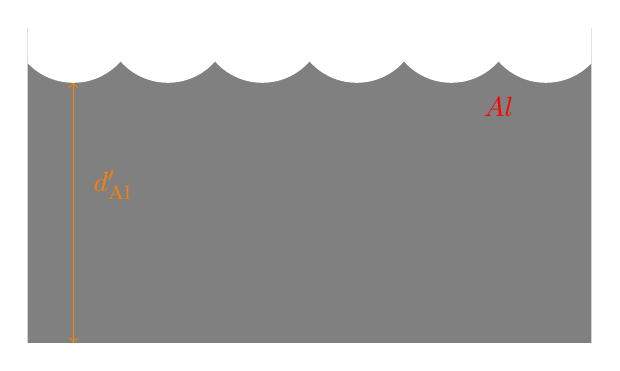
\begin{tikzpicture}
                \def\l{7.2};
                \def\h{4};
                \def\d{0.6};
                \begin{scope}
                    \clip (0.02,0) rectangle (\l - 0.02,\h);
                    \fill[gray] (0,0) rectangle (\l,\h);
                    \foreach \i in {1,3,...,11}{
                        \fill[white] (- 4 / 3 * \d + \i * \d, \h + 0.1) arc (180:360:\d / 3 * 4)--cycle;}
                    \draw[color=orange,<->] (0.6,0) -- (0.6,\h+0.1-0.8);
                    \node[color=orange] at (1.1,\h/2) {$d_\mathrm{Al}'$};
                    \node[color=red] at (6,3) {$\ce{Al}$};
                \end{scope}
            \end{tikzpicture}
            \label{fig:al-dissolution-1}}
        \hfill
        \subfloat[]{
        \tikzsetnextfilename{production_stage_4}
            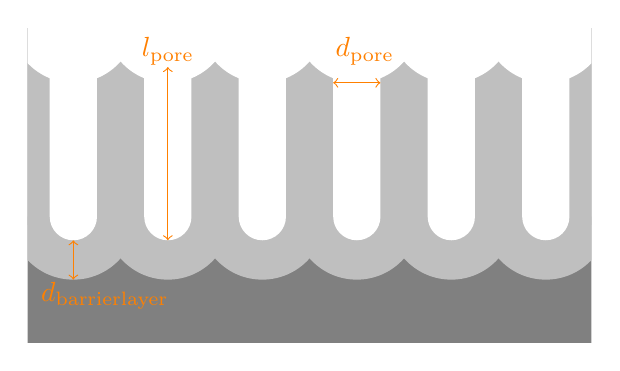
\begin{tikzpicture}
                \def\l{7.2};
                \def\h{4};
                \def\d{0.6};
                \begin{scope}
                \clip (0.02,0) rectangle (\l - 0.02,\h);
                \fill[gray] (0,0) rectangle (\l,\h);
                \fill[lightgray] (0,1.5) rectangle (\l,\h);
                \foreach \i in {1,3,...,11}{
                    \fill[white] (- 4 / 3 * \d + \i * \d, \h + 0.1) arc (180:360:\d / 3 * 4);
                    \fill[lightgray] (- 4 / 3 * \d + \i * \d, \h - 2.5 + 0.1) arc (180:360:\d / 3 * 4);
                    \fill[white] (-0.5 * \d + \i * \d, \h - 2.5 + 0.1) arc (180:360:\d / 2) -- (-0.5 * \d + \i * \d + \d, \h + 0.1) -- (-0.5 * \d + \i * \d, \h + 0.1) -- cycle;}
                \draw[color=orange,<->] (3.9,3.3) -- (4.5,3.3);
                \node[color=orange] at (4.3,3.7) {$d_\mathrm{pore}$};
                \draw[color=orange,<->] (0.6,\h-2.5+0.1-0.3) -- (0.6,\h-2.5+0.1-0.8);
                \node[color=orange] at (1,\h-2.5+0.1-0.8-0.2) {$d_\mathrm{barrier layer}$};
                \draw[color=orange,<->] (1.8,\h-2.5+0.1-0.3) -- (1.8,\h-+0.1-0.4);
                \node[color=orange] at (1.8,\h-0.3) {$l_\mathrm{pore}$};
                \end{scope}
            \end{tikzpicture}
            \label{fig:second-anodizing}}
        \\
        \subfloat[]{
        \tikzsetnextfilename{production_stage_5}
            
\begin{tikzpicture}
                \def\l{7.2};
                \def\h{3.5};
                \def\d{0.6};
                \begin{scope}
                \clip (0.02,0) rectangle (\l - 0.02,\h);
                %\fill[gray] (0,0) rectangle (\l,\h);
                \fill[lightgray] (0,1) rectangle (\l,\h);
                \foreach \i in {1,3,...,11}{
                    \fill[white] (- 4 / 3 * \d + \i * \d, \h + 0.1) arc (180:360:\d / 3 * 4);
                    \fill[lightgray] (- 4 / 3 * \d + \i * \d, \h - 2.5 + 0.1) arc (180:360:\d / 3 * 4);
                    \fill[white] (-0.5 * \d + \i * \d, \h - 2.5 + 0.1) arc (180:360:\d / 2) -- (-0.5 * \d + \i * \d + \d, \h + 0.1) -- (-0.5 * \d + \i * \d, \h + 0.1) -- cycle;}
                \end{scope}
            \end{tikzpicture}
            \label{fig:al-dissolution-2}}
        \hfill
        \subfloat[]{
        \tikzsetnextfilename{production_stage_6}
            
\begin{tikzpicture}
                \def\l{7.2};
                \def\h{3.5};
                \def\d{0.6};
                \begin{scope}
                \clip (0,0) rectangle (\l,\h);
                \fill[lightgray] (0,1.1) rectangle (\l,\h);
                \foreach \i in {1,3,...,11}{
                    \fill[white] (- 4 / 3 * \d + \i * \d, \h + 0.1) arc (180:360:\d / 3 * 4);
                    \fill[white] (-0.5 * \d + \i * \d, \h - 2.5 + 0.1) arc (180:360:\d / 2) -- (-0.5 * \d + \i * \d + \d, \h + 0.1) -- (-0.5 * \d + \i * \d, \h + 0.1) -- cycle;}
                \end{scope}
            \end{tikzpicture}
            \label{fig:barrier-layer-dissolution}}
        \caption{Production stages of the membrane production. It starts with a wafer of bulk aluminum (dark gray) \protect\subref{fig:bulk-al} which is then anodized yielding \protect\subref{fig:first-anodizing}, where light gray represents alumina. The latter is then dissolved producing a bulk aluminum wafer with hexagonally arranged hollows \protect\subref{fig:al-dissolution-1}. By the second anodizing, straight parallel pores are created \protect\subref{fig:second-anodizing}. After dissolving the remaining aluminum \protect\subref{fig:al-dissolution-2}, the barrier layer etched to open the pores \protect\subref{fig:barrier-layer-dissolution}. The initial aluminum wafer's thickness is $d_{\ce{Al}}=\SI{1}{\milli\meter}$, the \textit{barrier layer} thickness $d_\mathrm{barrier-layer}$ is $\SI{30}{\nano\meter}$
        to $\SI{60}{\nano\meter}$, the pore diameters $d_\mathrm{pore}=\SI{10}{\nano\meter}$ to $\SI{100}{\nano\meter}$ and the pore length or membrane thickness $l_\mathrm{pore}=\SI{30}{\micro\meter}$ to $\SI{60}{\micro\meter}$.}
        \label{fig:membrane-production}
    \end{figure}

\end{document}
